\noindent En este capítulo se exponen los experimentos realizados para demostrar la efectividad del estudio para clasificar ransomware. En la Sección \ref{sec:metricas} se listan las métricas usadas para detectar la efectividad del modelo. La Sección \ref{sec:experimentos} expone la elección de los parámetros más relevantes, se detallan los experimentos realizados en los dos \textit{datasets} y se muestran los resultados con diferentes algoritmos. En la Sección \ref{sec:resultados} se elegirá el algoritmo con mejor rendimiento y se compararán los resultados con los de los trabajos mencionados en el Capítulo \ref{Capitulo4}.

\section{Métricas Utilizadas}\label{sec:metricas}

\noindent Antes de explicar las métricas utilizadas, se deben definir los siguientes conceptos fundamentales:
\begin{itemize}
    \item \textbf{P}: Archivos ransomware.
    \item \textbf{N}: Archivos benignos.
    \item \textbf{\gls{TP}}: Número de archivos ransomware que han sido correctamente etiquetados como ransomware.
    \item \textbf{\gls{FP}}: Número de archivos benignos que han sido incorrectamente etiquetados como ransomware.
    \item \textbf{\gls{TN}}: Número de archivos benignos que han sido correctamente etiquetados como benignos.
    \item \textbf{\gls{FN}}: Número de archivos ransomware que han sido incorrectamente etiquetados como benignos.
    \item \textbf{Matriz de confusión}: Matriz mostrada en la Figura \ref{fig:matrix} donde se visualizan los conceptos anteriores para saber el rendimiento del algoritmo.
    
    \begin{figure}[h!]
    \begin{center}
    {\scalebox{.55}{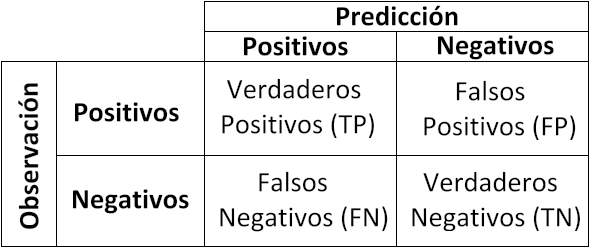
\includegraphics{images/matrix.png}}}
    \end{center}
    \caption{Matriz de confusión.}
    \label{fig:matrix} 
    \end{figure}
\end{itemize}

\newpage

A continuación se explicarán las métricas que se utilizarán en los experimentos:

\begin{itemize}
    \item \textbf{Precisión}: También conocida como \textit{accuracy}, es la proporción de archivos ransomware y benignos que han sido correctamente etiquetados.
    \begin{align*} Precisi\acute{o}n = \frac{\gls{TP} + \gls{TN}}{P + N} \end{align*}
    
    \item \textbf{Exactitud}: También conocida como \textit{precision}, es la proporción entre los positivos reales predichos por el algoritmo y todos los casos positivos.
    \begin{align*} Exactitud = \frac{\gls{TP}}{\gls{TP} + \gls{FP}} \end{align*}
    
    \item \textbf{Tasa de error}: Proporción de archivos ransomware y benignos etiquetados incorrectamente respecto al número total de archivos.  \begin{align*} ERR = \frac{\gls{FP} + \gls{FN}}{P + N} \end{align*}
    
    \item \textbf{\gls{TPR}}: También conocida como \textit{recall} o exhaustividad, es la proporción de archivos ransomware etiquetados correctamente.
    \begin{align*} \gls{TPR} = \frac{\gls{TP}}{\gls{TP} + \gls{FN}}\end{align*}
    
    \item \textbf{\gls{TNR}}: También conocida como \textit{specificity}, es la proporción de archivos benignos etiquetados correctamente.
    \begin{align*} \gls{TNR} = \frac{\gls{TN}}{\gls{TN} + \gls{FP}}\end{align*}
    
    \item \textbf{\gls{FPR}}: Proporción de archivos benignos etiquetados incorrectamente.
    \begin{align*} \gls{FPR} = \frac{\gls{FP}}{\gls{FP} + \gls{TN}} \end{align*}
    
    \item \textbf{\gls{FNR}}: Proporción de archivos ransomware etiquetados incorrectamente.
    \begin{align*} \gls{FNR} = \frac{\gls{FN}}{\gls{FN} + \gls{TP}} \end{align*}
    
    \item \textbf{Valor F}: También conocido como \textit{F1-score}, es la media harmónica de la exactitud y la exhaustividad o \gls{TPR}.
    \begin{align*} Valor\,F = 2 \cdot\frac{exactitud \cdot exhaustividad}{exactitud + exhaustividad} \end{align*} 
\end{itemize}


\section{Experimentos} \label{sec:experimentos}

\noindent Los experimentos se han realizado sobre los dos \textit{datasets} explicados en la Sección \ref{sec:features} y se han extraído todas las métricas detalladas en la Sección \ref{sec:metricas}. Como bien se ha mencionado en la Sección \ref{sec:model}, se ha utilizado el lenguaje de programación Python y la librería ``scikit-learn'' \cite{scikit-learn} para el desarrollo de los experimentos, y para la visualización de las gráficas se ha usado ``matplotlib'' \cite{matplotlib}.


\subsection{Ajustar Parámetros} \label{adjust}
\noindent Primero se realizan una serie de pruebas sobre los \textit{datasets} para obtener los parámetros que mejor precisión vayan a proporcionar a nuestros experimentos. Los parámetros a estudiar son: 
\begin{itemize}
    \item Método de escalado utilizado: Debido a que el \textit{dataset suma} posee un rango muy amplio de valores, se decide llevar a cabo una estandarización de los datos, de manera que el modelo se comporte de una manera más eficiente y se obtenga un mayor rendimiento. Para ello, en este estudio se proponen dos métodos de la librería de Python ``sci-kit learn''. Por un lado, la función \textit{StandardScaler()}, estandariza los valores de X restando la media y luego escalando a la varianza de la unidad, mientras que \textit{MinMaxScaler()}, escala las características a un rango dado, en este caso [0,1]. Mediante la Figura \ref{fig:compsuma3}, es posible observar una mayor precisión en los algoritmos utilizando la función \textit{StandardScaler()}. 
    
    \begin{figure}[h!]
    \begin{center}
    {\scalebox{.53}{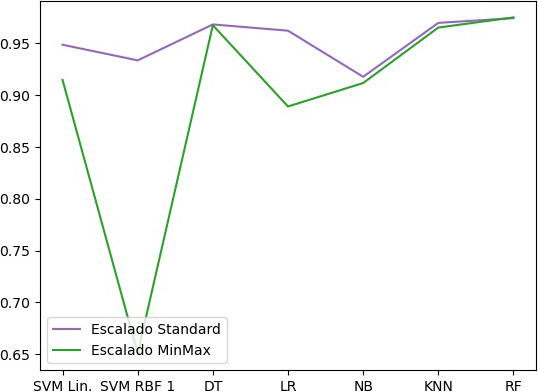
\includegraphics{images/ComparacionEscalado.jpg}}}
    \end{center}
    \caption{Comparación de la precisión con distintos métodos de escalado usando el \textit{dataset suma}}
    \label{fig:compsuma3}
    \end{figure}
    
    \item Valor de K en la validación cruzada: Para la validación mediante la técnica K-Fold se utilizan 3 valores distinto para tratar de obtener el mejor resultado posible. Las Figuras \ref{fig:compbin2} y \ref{fig:compsuma2} dan constancia de un mejor comportamiento para K=10 en ambos \textit{datasets}, por lo tanto será el valor usado en los experimentos que utilicen validación cruzada.
    
    \begin{figure}[htb!]
    \begin{center}
    \subfigure[Precisión en \textit{dataset binario}]{
        {\scalebox{.52}{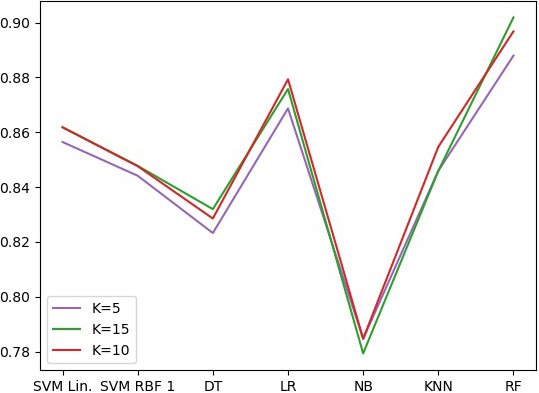
\includegraphics{images/ComparacionKFoldBinario.jpg}}}
        \label{fig:compbin2}}
    \subfigure[Precisión en \textit{dataset suma}]{
        {\scalebox{.52}{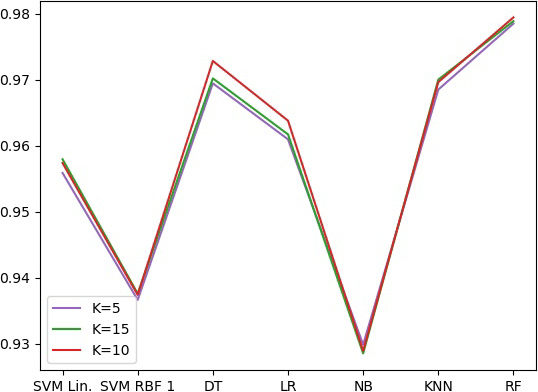
\includegraphics{images/ComparacionKFoldSuma.jpg}}}
        \label{fig:compsuma2}}
    \caption{Comparación de la precisión con distintos valores de K en validación cruzada K-fold usando en los dos \textit{datasets}}
    \label{fig:comp_kfold}
    \end{center}
    \end{figure}
    
    \item Distribución del \textit{dataset}: Se realizan experimentos para utilizar una proporción óptima entre los datos de entrenamiento y los datos de prueba. Como se puede observar en las Figuras \ref{fig:compbin1} y \ref{fig:compsuma1}, se decide utilizar un 70\% de los datos para el entrenamiento del modelo y un 30\% para las pruebas, puesto que reflejan una mayor precisión tanto en el \textit{dataset suma} como en el \textit{dataset binario}.
    
    \begin{figure}[htb!]
    \begin{center}
    \subfigure[Precisión en \textit{dataset binario}]{
        {\scalebox{.52}{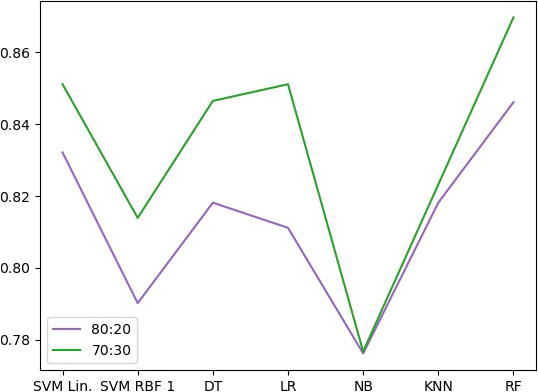
\includegraphics{images/ComparacionTestBinario.jpg}}}
        \label{fig:compbin1}}
    \subfigure[Precisión en \textit{dataset suma}]{
        {\scalebox{.52}{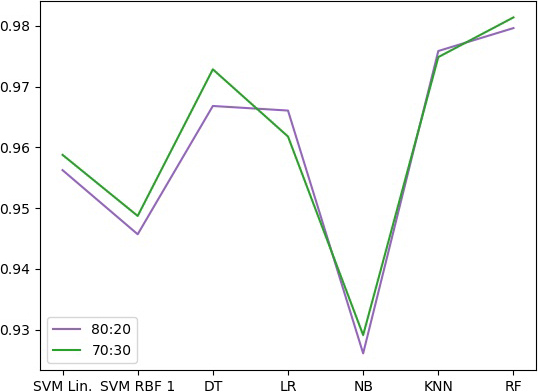
\includegraphics{images/ComparacionTestSuma.jpg}}}
        \label{fig:compsuma1}}
    \caption{Comparación de la precisión con distintas distribuciones de los dos \textit{datasets}}
    \label{fig:comp_distrib}
    \end{center}
    \end{figure}
    
    
\end{itemize}


\subsection{Experimentos con el \textit{Dataset binario}} \label{sec:exp1}

\noindent El primer \textit{dataset} es el llamado \textit{dataset binario}, que contiene los archivos y las \gls{API}s a las que llama (1 si llama a esa \gls{API}, 0 si no). Para realizar los experimentos, se utiliza un script de Python para entrenar los datos y realizar las predicciones. Posteriormente, dicho script genera una serie de gráficas para visualizar los resultados y poder decidir qué algoritmo y qué configuración es la deseada para construir el modelo.

Todos los resultados de las métricas analizadas pueden observarse en la Tabla \ref{tab:rto_binario_nokfold}. Se puede apreciar que el algoritmo con le mejor rendimiento es \gls{RF} por tener la precisión y el valor f más altos, unas tasas verdaderas (\gls{TPR} y \gls{TNR}) altas y tasas falsas bajas (\gls{FPR} y \gls{FNR}), lo que significa que el algoritmo ha sido capaz de clasificar las muestras con pocos errores, hecho que se confirma con su tasa de error, que es la más baja de todas (0.041).

\begin{table}[h!]
    \centering
    \scriptsize %para hacer la tabla mas pequeña
    \caption{Resultados con el \textit{dataset binario}.}
    \begin{tabular}{|c|c|c|c|c|c|c|c|c|}
        \hline
        \rowcolor[HTML]{C0C0C0} 
        \textbf{Algoritmo} & \textbf{Precisión} & \textbf{Exactitud} & \textbf{Valor F} & \textbf{\gls{TPR}} & \textbf{\gls{TNR}} & \textbf{\gls{FPR}} & \textbf{\gls{FNR}} & \textbf{Tasa de Error}\\ \hline
        
        \gls{SVM} Lineal & 0.86 & 0.89 & 0.86 & 0.84 & 0.88 & 0.12 & 0.16 & 0.042\\ \hline
        \gls{SVM} \gls{RBF} & 0.82 & 0.91 & 0.81 & 0.72 & 0.92 & 0.09 & 0.25 & 0.055 \\ \hline
        \gls{DT} & 0.83 & 0.88 & 0.83 & 0.79 & 0.88 & 0.12 & 0.21 & 0.050\\ \hline
        \gls{LR} & 0.85 & 0.89 & 0.85 & 0.80 & 0.89 & 0.11 & 0.2 & 0.045\\ \hline
        \gls{NB} & 0.73 & 0.89 & 0.68 & 0.55 & 0.92 & 0.11 & 0.34 & 0.081\\ \hline
        \gls{KNN} & 0.8 & 0.89 & 0.79 & 0.71 & 0.90 & 0.11 & 0.26 & 0.056\\ \hline
        \gls{RF} & 0.87 & 0.90 & 0.87 & 0.83 & 0.90 & 0.09 & 0.17 & 0.041\\ \hline
        
    \end{tabular}
    \label{tab:rto_binario_nokfold}
\end{table}

\newpage

Las gráficas de barras de las Figuras \ref{fig:comp_precision}, \ref{fig:comp_exactitud} y \ref{fig:comp_recall} permiten comparar la precisión, la exactitud y la exhaustividad (\gls{TPR}) de los algoritmos del modelo al usar o no la validación K-Fold.

\begin{figure}[h!]
    \begin{center}
    \subfigure[Precisión sin validación K-fold]{
        {\scalebox{.5}{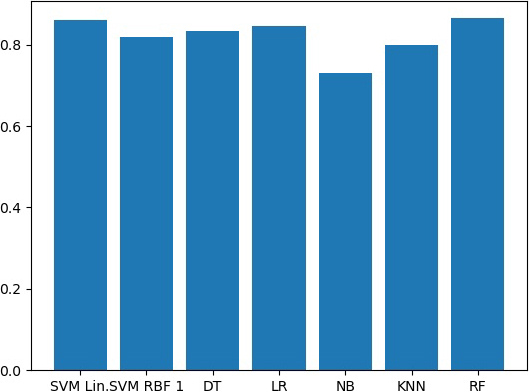
\includegraphics{images/PrecisionBinario3.jpg}}}
        \label{fig:precision_bin1}}
    \subfigure[Precisión con validación K-fold]{
        {\scalebox{.5}{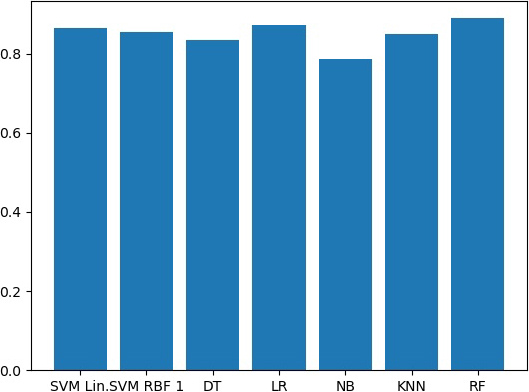
\includegraphics{images/PrecisionBinarioKF3.jpg}}}
        \label{fig:precision_bin2}}
    \caption{Comparación de la precisión con y sin validación k-fold de todos los algoritmos en \textit{dataset binario}}
    \label{fig:comp_precision}
    \end{center}
\end{figure}

\begin{figure}[h!]
    \begin{center}
    \subfigure[Exactitud sin validación K-fold]{
        {\scalebox{.5}{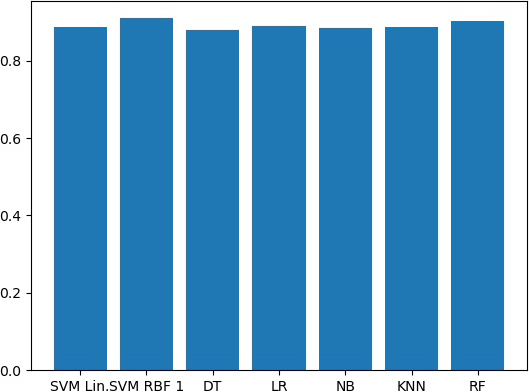
\includegraphics{images/ExactitudBinario3.jpg}}}
        \label{fig:exactitud_bin1}}
    \subfigure[Exactitud con validación K-fold]{
        {\scalebox{.5}{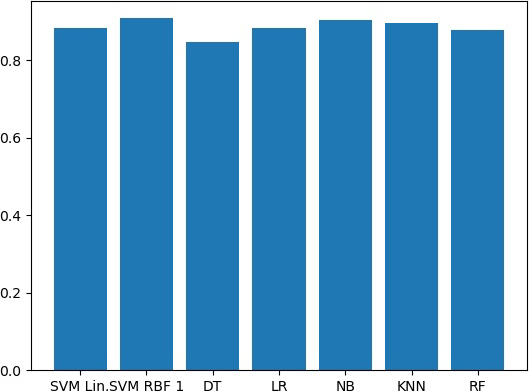
\includegraphics{images/ExactitudBinarioKF3.jpg}}}
        \label{fig:exactitud_bin2}}
    \caption{Comparación de la exactitud con y sin validación k-fold de todos los algoritmos en \textit{dataset binario}}
    \label{fig:comp_exactitud}
    \end{center}
\end{figure}

\begin{figure}[h!]
    \begin{center}
    \subfigure[\gls{TPR} sin validación K-fold]{
        {\scalebox{.5}{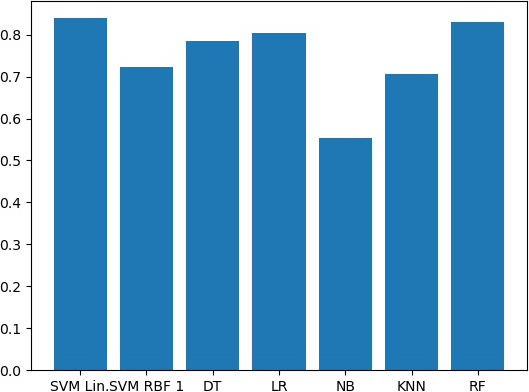
\includegraphics{images/RecallBinario3.jpg}}}
        \label{fig:exactitud_rec1}}
    \subfigure[\gls{TPR} con validación K-fold]{
        {\scalebox{.5}{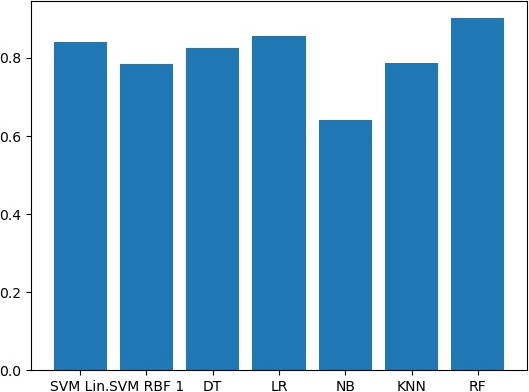
\includegraphics{images/RecallBinarioKF3.jpg}}}
        \label{fig:exactitud_rec2}}
    \caption{Comparación de la TPR con y sin validación k-fold de todos los algoritmos en \textit{dataset binario}}
    \label{fig:comp_recall}
    \end{center}
\end{figure}


Los resultados no varían demasiado al usar o no la validación K-fold, y hasta algunos algoritmos rinden mejor sin usarla, como es el caso de \gls{RF}, \gls{LR} y \gls{DT} con la precisión y exactitud, y de \gls{SVM} Linear con la \gls{TPR}. Con esto se garantiza que nuestro modelo es válido, ya que los resultados son independientes de la partición de datos de prueba y entrenamiento. Se concluye que los mejores resultados se obtienen con el algoritmo \gls{RF}.


\subsection{Experimentos con el \textit{Dataset suma}} \label{sec:exp2}

\noindent El segundo \textit{dataset} es el llamado \textit{dataset suma}, que contiene los archivos y el número de veces que llama a las \gls{API}s. Al igual que para el \textit{dataset} anterior, se utiliza un \textit{script} muy similar, pero se añade la estandarización de las características para reducir el tiempo de cómputo.


En la Tabla \ref{tab:rto_suma_nokfold} se muestras todos los datos obtenidos en los experimentos realizados para el \textit{dataset suma}. Al igual que sucedió con el primer \textit{dataset}, el algoritmo que da mejores resultados es \gls{RF}, siendo mejor que los demás en todas las métricas exceptuando la tasa de falsos positivos \gls{FPR} con un valor de 0.026, pero la diferencia con la mejor, que es 0.020 con el algoritmo \gls{SVM} \gls{RBF}, es mínima.

\begin{table}[h!]
    \centering
    \scriptsize %para hacer la tabla mas pequeña
    \caption{Resultados con el \textit{dataset suma} escalando los datos con \textit{StandardScaler}.}
    \begin{tabular}{|c|c|c|c|c|c|c|c|c|}
        \hline
        \rowcolor[HTML]{C0C0C0} 
        \textbf{Algoritmo} & \textbf{Precisión} & \textbf{Exactitud} & \textbf{Valor F} & \textbf{\gls{TPR}} & \textbf{\gls{TNR}} & \textbf{\gls{FPR}} & \textbf{\gls{FNR}} & \textbf{Tasa de Error}\\ \hline
        
        \gls{SVM} Lineal & 0.95 & 0.96 & 0.95 & 0.95 & 0.96 & 0.04 & 0.051 & 0.014\\ \hline
        \gls{SVM} \gls{RBF} & 0.95 & 0.93 & 0.95 & 0.96 & 0.93 & 0.068 & 0.041 & 0.021\\ \hline
        \gls{DT} & 0.98 & 0.98 & 0.97 & 0.97 & 0.98 & 0.020 & 0.03 & 0.008\\ \hline
        \gls{LR} & 0.96 & 0.97 & 0.96 & 0.95 & 0.97 & 0.03 & 0.05 & 0.012\\ \hline
        \gls{NB} & 0.92 & 0.97 & 0.91 & 0.87 & 0.97 & 0.03 & 0.12 & 0.024\\ \hline
        \gls{KNN} & 0.97 & 0.98 & 0.97 & 0.96 & 0.98 & 0.23 & 0.036 & 0.009\\ \hline
        \gls{RF} & 0.98 & 0.97 & 0.98 & 0.99 & 0.97 & 0.026 & 0.013 & 0.006\\ \hline
        
    \end{tabular}
    \label{tab:rto_suma_nokfold}
\end{table}

\newpage

Las Figuras \ref{fig:comp_p_suma}, \ref{fig:comp_e_suma} y \ref{fig:comp_r_suma} muestran las diferencias en las métricas de precisión y exactitud tras usar o no la validación K-Fold. Como se ha visto en el primer \textit{dataset}, los resultados al usar o no la validación no son muy diferentes, y en algoritmos como \gls{RF} y \gls{DT} los resultados son mejores sin la validación cruzada. Una vez más se demuestra la validez del modelo, gracias a que los resultados con y sin validación son muy similares.

\begin{figure}[h!]
    \begin{center}
    \subfigure[Precisión sin validación K-fold]{
        {\scalebox{.5}{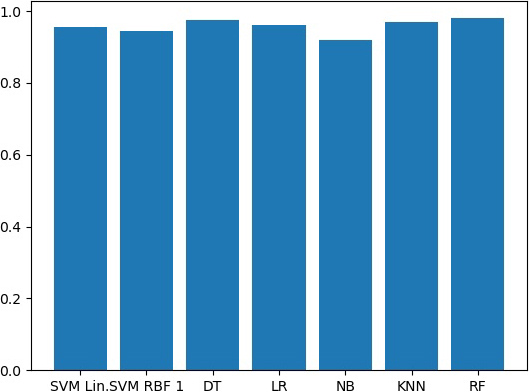
\includegraphics{images/PrecisionSuma3.jpg}}}
        \label{fig:precision_suma1}}
    \subfigure[Precisión con validación K-fold]{
        {\scalebox{.5}{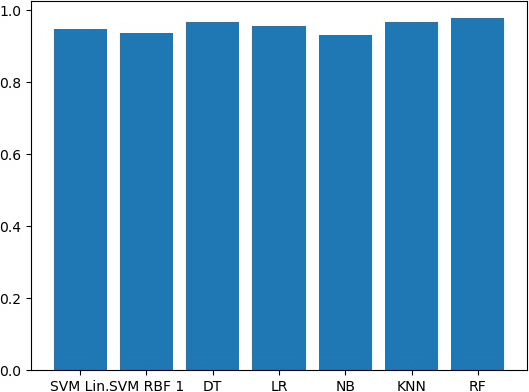
\includegraphics{images/PrecisionSumaKF3.jpg}}}
        \label{fig:precision_suma2}}
    \caption{Comparación de la precisión con y sin validación k-fold de todos los algoritmos en \textit{dataset suma}}
    \label{fig:comp_p_suma}
    \end{center}
\end{figure}

\begin{figure}[h!]
    \begin{center}
    \subfigure[Exactitud sin validación K-fold]{
        {\scalebox{.5}{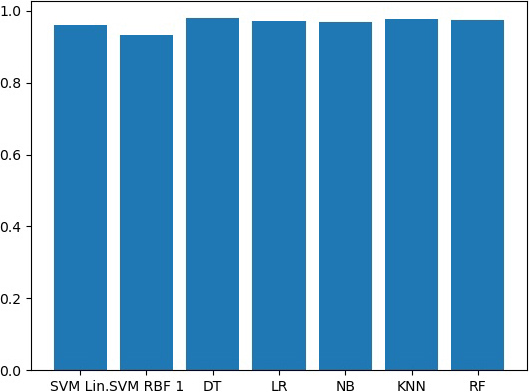
\includegraphics{images/ExactitudSuma3.jpg}}}
        \label{fig:exactitud_bin3}}
    \subfigure[Exactitud con validación K-fold]{
        {\scalebox{.5}{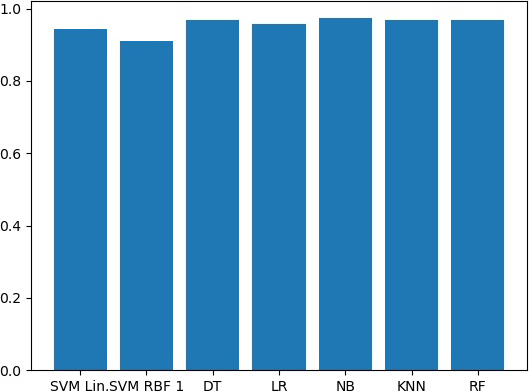
\includegraphics{images/ExactitudSumaKF3.jpg}}}
        \label{fig:exactitud_bin4}}
    \caption{Comparación de la exactitud con y sin validación k-fold de todos los algoritmos en \textit{dataset suma}}
    \label{fig:comp_e_suma}
    \end{center}
\end{figure}

\begin{figure}[h!]
    \begin{center}
    \subfigure[\gls{TPR} sin validación K-fold]{
        {\scalebox{.5}{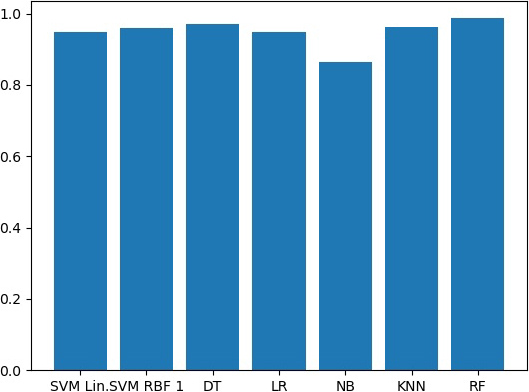
\includegraphics{images/RecallSuma3.jpg}}}
        \label{fig:exactitud_rec3}}
    \subfigure[\gls{TPR} con validación K-fold]{
        {\scalebox{.5}{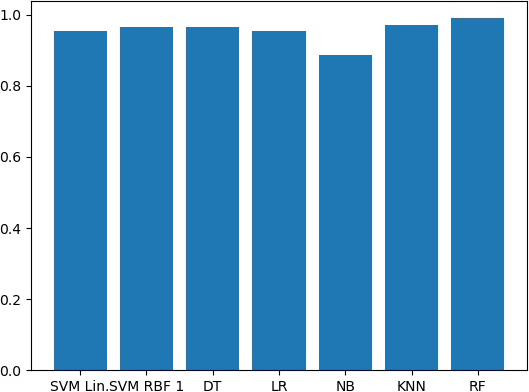
\includegraphics{images/RecallSumaKF3.jpg}}}
        \label{fig:exactitud_rec4}}
    \caption{Comparación de la TPR con y sin validación k-fold de todos los algoritmos en \textit{dataset suma}}
    \label{fig:comp_r_suma}
    \end{center}
\end{figure}

\newpage

Al igual que con el primer \textit{dataset}, se concluye que el algoritmo más eficiente y con los mejores resultados es \gls{RF}.

\section{Resultados Finales} \label{sec:resultados}

%PONER AQUI EL MEJOR ALGORITMO Y DECIR QUE CON ESE CREAMOS NUESTRO MODELO

%poner aqui la comparación de los experimentos con otros trabajos comentados en el capitulo de estado del arte

\noindent Como se ha visto en las Secciones \ref{sec:exp1} y \ref{sec:exp2}, el algoritmo con los mejores resultados es \gls{RF}, usando el \textit{dataset suma} distribuido de manera que el 70\% de los datos se usen para el entrenamiento del modelo y un 30\% para las pruebas. Con todo esto en cuenta, se generará el modelo final de este trabajo.

A continuación se muestran la Tabla \ref{tab:comparacion} que compara los resultados del modelo final de este trabajo con los resultados de los otros trabajos que usan el algoritmo \gls{RF}, vistos en la Tabla \ref{tab:estadoarte} del Capitulo \ref{Capitulo4}. Se puede apreciar que los resultados de este trabajo están entre los mejores, teniendo las menores tasas de falsos positivos y negativos (\gls{FPR} y \gls{FNR}), la segunda mejor tasa de verdaderos positivos (\gls{TPR}) y unos valores de precisión y valor F bastante altos, demostrando la efectividad del modelo propuesto.

%COMPARAR CON LOS RANDOM FOREST DE LOS OTROS TRABAJOS
\begin{table}[htb!]
    \centering
    \scriptsize %para hacer la tabla mas pequeña
    \caption{Comparación de los resultados obtenidos con otros trabajos usando el algoritmo RF}
    \begin{tabular}{|c|c|c|c|c|c|c|c|c|}
        \hline
        \rowcolor[HTML]{C0C0C0} 
        \textbf{Trabajo} & \textbf{Precisión} & \textbf{Exactitud} & \textbf{Valor F} & \textbf{\gls{TPR}} & \textbf{\gls{TNR}} & \textbf{\gls{FPR}} & \textbf{\gls{FNR}} & \textbf{Tasa de Error}\\ \hline
        
        \cite{shallow} (2017) & 0.98 & 0.98 & 0.99 & 1.0 & - & - & - & -\\ \hline
        \cite{flow} (2017) & 0.958 & - & - & 0.96 & - & 0.047 & - & -\\ \hline
        \cite{detecting} (2019) & 0.98 & 0.98 & 0.98 & 0.98 & - & - & - & -\\ \hline
        \cite{Kok2019} (2019) & 0.92 & - & - & 0.91 & - & 0.07 & - & -\\ \hline
        \cite{entropy} (2019) & 0.97 & - & 0.97 & 0.97 & - & - & - & -\\ \hline
        \cite{two} (2020) & 0.973 & - & 0.97 & - & - & 0.048 & 0.015 & -\\ \hline
        \cite{Kok2020} (2020) & 0.99 & - & 0.99 & 0.99 & - & - & - & -\\ \hline
        \cite{ARABO2020289} (2020) & 0.75 & - & - & - & - & - & - & -\\ \hline
        \cite{Aurangzeb2021} (2021) & 0.97 & - & 0.97 & 0.94 & - & - & - & -\\ \hline
        Este trabajo & 0.98 & 0.97 & 0.98 & 0.99 & 0.97 & 0.026 & 0.013 & 0.006\\ \hline
        
    \end{tabular}
    \label{tab:comparacion}
\end{table}

\newpage

%%COMENTAR TODO

%alzar nuestros resultados aunque sean peores, pero como hacemos con mas muestras pues es mejor, ya que nosotros usamos muuchas muestras y eso esta bien

La Tabla \ref{tab:comparacionDatasets} coteja el \textit{dataset} construido en este trabajo con el de los demás trabajos. 

\begin{table}[htb!]
    \centering
    \scriptsize %para hacer la tabla mas pequeña
    \caption{Comparación de los \textit{datasets} construidos con los del estado del arte}
    \label{tab:comparacionDatasets}
    \begin{tabular}{|p{0.17\textwidth}|p{0.5\textwidth}|p{0.24\textwidth}|}
        \hline
        \rowcolor[HTML]{C0C0C0}
        \multicolumn{1}{|c|}{\cellcolor[HTML]{C0C0C0}{\textbf{Trabajo}}} &
        \multicolumn{1}{c|}{\cellcolor[HTML]{C0C0C0}{\textbf{Distribución de las muestras}}} &
        \multicolumn{1}{c|}{\cellcolor[HTML]{C0C0C0}{\textbf{Tamaño total}}} \\ \hline
        \cite{shallow} (2017) & 755 muestras de ransomware y 219 muestras benignas & 974 \\ \hline
        \cite{flow} (2017) & 83 muestras de ransomware y 85 muestras benignas & 168 \\ \hline
        \cite{detecting} (2019) & \textit{Dataset} conformado por 1000 muestras de ransomware, 900 muestras de malware y 300 muestras benignas & 2200\\ \hline
        \cite{Kok2019} (2019) & 582 muestras de ransomware y 942 muestras benignas & 1524 \\ \hline
        \cite{entropy} (2019) & 1072 muestras de ransomware y 1072 muestras benignas generadas sintéticamente a partir de un \textit{dataset} real de 663 muestras ransomware y 103 muestras benignas & 2144\\ \hline
        \cite{two} (2020) & 1909 muestras de ransomware y 1139 muestras benignas & 3048 \\ \hline
        \cite{Kok2020} (2020) & 904 muestras de ransomware y 942 muestras benignas. & Eliminando repetidos, al igual que en este estudio, se obtiene un \textit{dataset} final de 912 muestras totales. \\ \hline
        \cite{ARABO2020289} (2020) & 34 muestras de malware, de las cuales 7 son ransomware, y 41 muestras benignas & 75 \\ \hline
        \cite{Aurangzeb2021} (2021) & 80 muestras de ransomware y 80 muestras de otros tipos de malware & 160 \\ \hline
        \multirow{2}{*}{Este trabajo} & \textit{Dataset} binario: mitad ransomware mitad benigno. Representada la aparición de las \gls{API} en formato binario & 714 \\ \cline{2-3}& \textit{Dataset} suma: Muestras ransomware y benignas a partes iguales. Representando la aparición de las \gls{API} por el número de llamadas. & 6630 \\ \hline
    \end{tabular}
\end{table}

Los datos reflejan la superioridad en tamaño del \textit{dataset} conformado en este trabajo, en concreto el segundo \textit{dataset}, con un número total de 6630 muestras, que es el que se ha usado para obtener los mejores resultados. Además, gracias a la cortesía de S.H. Kok \textit{et al.} en \cite{Kok2020}, se han podido hacer pruebas con el \textit{dataset} que utilizan en el trabajo. Tras realizar el proceso de limpieza de su \textit{dataset} con el sistema propuesto, se reducen las muestras casi al 50\%. Se puede asumir por lo tanto, que el \textit{dataset} del modelo propuesto, a parte de ser mayor, es menos propenso al \textit{overfitting}, debido a que no aparecen muestras repetidas en ningún caso. 

Por otro lado, al utilizar dos \textit{datasets} diferentes, se proporcionan dos enfoques distintos, realizando así un estudio más completo. Con toda esta información, y debido a unos resultados muy favorables vistos en la Tabla \ref{tab:comparacion}, %ES SOLO UNA IDEA, HABRIA QUE CONSULTAR 
se puede afirmar que se obtiene una mayor precisión en la identificación de ransomware al utilizar una mayor cantidad de muestras, con un equilibrio entre las muestras benignas y de ransomware y recogiendo la cantidad de llamadas a las \gls{API} de Windows en lugar de utilizar su aparición.